\documentclass{amsart}
\synctex=1

\newcount\DraftStatus  % 0 suppresses notes to selves in text
\DraftStatus=1

\usepackage{comment}

\includecomment{JournalOnly}  
\includecomment{ConferenceOnly}  
\includecomment{TulipStyle}

%=================================================================
% gitlatexdiff
%
%  https://gitlab.com/git-latexdiff/git-latexdiff
%=================================================================
%  git latexdiff HEAD  HEAD~5 --main templatex.tex
%  git latexdiff HEAD~1  --main templatex.tex
%  View pdf to see difference
%
%=================================================================
%
% Todo Notes for marginal comments
% 
%\newcount\DraftStatus  % 0 suppresses notes to selves in text
%\DraftStatus=1   % TODO: set to 0 for final version
\ifnum\DraftStatus=1
	\usepackage[draft,colorinlistoftodos,color=orange!30]{todonotes}
\else
	\usepackage[disable,colorinlistoftodos,color=blue!30]{todonotes}
\fi 
%\usepackage[disable]{todonotes} % notes not showed
%\usepackage[draft]{todonotes}   % notes showed
%
\makeatletter
 \providecommand\@dotsep{5}
 \def\listtodoname{List of Todos}
 \def\listoftodos{\@starttoc{tdo}\listtodoname}
 \makeatother
%
%=================================================================
%
\usepackage{color}
\newcommand{\draftnote}[3]{ 
	\todo[author=#2,color=#1!30,size=\footnotesize]{\textsf{#3}}	}
% TODO: add yourself here:
%
\newcommand{\gangli}[1]{\draftnote{blue}{GLi:}{#1}}
\newcommand{\qwu}[1]{\draftnote{red}{QWu:}{#1}}
\newcommand{\gliMarker}
	{\todo[author=GLi,size=\tiny,inline,color=blue!40]
	{Gang Li has worked up to here.}}
\newcommand{\qwuMarker}
	{\todo[author=QWu,size=\tiny,inline,color=red!40]
	{Qiong Wu has worked up to here.}}
%=================================================================

%=================================================================
%
% general packages
%  https://en.wikibooks.org/wiki/Category:Book:LaTeX
%  https://en.wikibooks.org/wiki/LaTeX/Package_Reference
%
%=================================================================
\usepackage{graphicx}
\graphicspath{{./figures/}{./graphics/}{./graphics/logos/}}

\usepackage{algorithm}
\usepackage{algorithmic}
\usepackage{breqn}
\usepackage{subcaption}
\usepackage{multirow}
\usepackage{psfrag}
\usepackage{url}
\usepackage[colorlinks,citecolor=blue]{hyperref}
%\usepackage{hyperref}
%\usepackage[colorlinks]{hyperref}
%\usepackage{cite}
\usepackage{cleveref}
\usepackage{booktabs}
\usepackage{rotating}
\usepackage{colortbl}
\usepackage{paralist}
%\usepackage{geometry}
\usepackage{epstopdf}
\usepackage{nag}
\usepackage{microtype}
\usepackage{siunitx}
\usepackage{nicefrac}
%\usepackage{breakurl}
\usepackage{fontawesome}
\usepackage{xcolor}
\usepackage{multicol}
\usepackage{wrapfig}
\usepackage{todonotes}
\usepackage{tablefootnote}
\usepackage{threeparttable}
% \usepackage{bibunits} 
% for random text
\usepackage{cite}
\usepackage{lipsum}
\usepackage[english]{babel}
\usepackage[pangram]{blindtext}
% for tikz figures
\usepackage{tikz}
\usetikzlibrary{fit,positioning,arrows.meta,shapes,arrows}
%\tikzset{neuron/.style={circle,thick,fill=black!25,minimum size=17pt,inner sep=0pt},
%	input neuron/.style={neuron, draw,thick, fill=gray!30},
%	hidden neuron/.style={neuron,fill=white,draw},
%	hoz/.style={rotate=-90}}
%
%=================================================================



\begin{TulipStyle}
\usepackage[numbers]{natbib}
%=================================================================
%
% Version control information
%
%=================================================================
\usepackage{gitinfo2}
%=================================================================
\usepackage{fancyhdr}
\pagestyle{fancy}
\fancyhead{} % clear all header fields
\fancyhead[RO,LE]{\textsl{\rightmark}}
\fancyhead[LO,RE]{\ensuremath{\Rightarrow}
		\textbf{\textbf{[CONFIDENTIAL]}}\ensuremath{\Leftarrow}}
\fancyhead[CO,CE]{}
%=================================================================
\fancyfoot{} % clear all footer fields
\fancyfoot[CE,CO]{\textbf{\thepage}} 
\fancyfoot[LO,LE]{
\includegraphics[height=.9\headheight]
{./graphics/logos/tulip-logo.eps}
		\gitVtagn-\gitBranch\ (\gitCommitterDate)}
\fancyfoot[RO,RE]{Committed by: \textsl{\gitCommitterName}}

\setlength{\headheight}{12pt}
\renewcommand{\headrulewidth}{0.4pt}
\renewcommand{\footrulewidth}{0.4pt}
%=================================================================


%=================================================================
% for math notations
% ----------------------------------------------------------------
\usepackage{mathtools}
\usepackage{amsthm}
%
% THEOREMS -------------------------------------------------------
%
\newtheorem{thm}{Theorem}[section]
\newtheorem{cor}[thm]{Corollary}
\newtheorem{lem}[thm]{Lemma}
\newtheorem{prop}[thm]{Proposition}
\theoremstyle{definition}
\newtheorem{defn}[thm]{Definition}
\theoremstyle{remark}
\newtheorem{rem}[thm]{Remark}
\numberwithin{equation}{section}
% MATH -----------------------------------------------------------
\newcommand{\norm}[1]{\left\Vert#1\right\Vert}
\newcommand{\abs}[1]{\left\vert#1\right\vert}
\newcommand{\set}[1]{\left\{#1\right\}}
\newcommand{\Real}{\mathbb R}
\newcommand{\eps}{\varepsilon}
\newcommand{\To}{\longrightarrow}
\newcommand{\BX}{\mathbf{B}(X)}
% ----------------------------------------------------------------
\newcommand{\I}{{\cal I}}
\newcommand{\Id}{{\cal I} }
\newcommand{\Dc}{{\cal D}}
\newcommand{\J}{{\cal J}}
\newcommand{\Dn}{{\cal D}_n}
\newcommand{\Dd}{{\cal D}_n }
\renewcommand{\P}{{\cal P}}
\newcommand{\Nu}{{\cal N} }
\newcommand{\B}{{\cal B}}
\newcommand{\Bf}{{\bf B}}
\newcommand{\Y}{{\bf Y}}
\newcommand{\A}{{\cal A}}
% ----------------------------------------------------------------
\newcommand{\V}{{\cal V}}
\newcommand{\M}{{\cal M}}
\newcommand{\F}{{\cal F}}
\newcommand{\Fd}{{\cal F}}
\newcommand{\BF}{{\cal BF}_n}
\newcommand{\BFd}{{\cal BF}_n}
\newcommand{\TF}{{\cal TF}_n}
\newcommand{\TFd}{{\cal TF}_n}
%\newcommand{\G}{{\cal G}}
\newcommand{\X}{{\cal X}}
\newcommand{\E}{{\cal E}}
\newcommand{\K}{{\cal K}}
\newcommand{\T}{{\cal T}_n}
\renewcommand{\H}{{\cal H}}
% ----------------------------------------------------------------
\newtheorem{Remark}{Remark}
\newtheorem{proposition}{Proposition}
\newtheorem{theorem}{Theorem}
\newtheorem{lemma}{Lemma}
\newtheorem{corollary}{Corollary}
\newtheorem{example}{Example}
\newtheorem{definition}{Definition}
\newtheorem{Algorithms}{Algorithm}
% ----------------------------------------------------------------
\newcommand{\bu}{{\mathbf 1} }
\newcommand{\bo}{{\mathbf 0} }
\newcommand{\N}{\mbox{{\sl l}}\!\mbox{{\sl N}}}
% ----------------------------------------------------------------
\def\uint{[0,1]}
\def\proof{{\scshape Proof}. \ignorespaces}
\def\endproof{{\hfill \vbox{\hrule\hbox{%
   \vrule height1.3ex\hskip1.0ex\vrule}\hrule
  }}\par}
%
%=================================================================

\hypersetup
{
    pdfauthor={\gitAuthorName},
    pdfsubject={TULIP Lab},
    pdftitle={},
    pdfkeywords={TULIP Lab, Data Science},
%	bookmarks=true,  
}

\end{TulipStyle}



\begin{document}
	\title[A Short Running Title]{Data Forecasting Project Report\\{\small House Prices-Advanced Regression Techniques}}%
	\author{Tao Wang}
	\date{\today}
	\maketitle
	
	\section{Project Description}\label{sec-intro}
	For home buyers, they generally do not buy homes with basements or near railroads, and there are other features of a home that can even much more influence the price of a home than the number of bedrooms. This project provides 79 characteristics of a house that are used to predict the price of a house.
	\section{Project Evaluation}\label{sec-intro}
	There are 1459 data in the test set, and the output contains ID numbers and predicted house prices. Submissions are evaluated on Root-Mean-Squared-Error (RMSE) between the logarithm of the predicted value and the logarithm of the observed sales price.
	\section{Dataset Description}\label{sec-intro}
	\subsection{File Description}\label{sec-intro}
	\begin{itemize}
		\item train.csv - the training set
		\item test.csv - the test set
		\item data_description.txt - full description of each column, originally prepared by Dean De Cock but lightly edited to match the column names used here
		\item sample_submission.csv - a benchmark submission from a linear regression on year and month of sale, lot square footage, and number of bedrooms
	\end{itemize}
	\subsection{Data fields}\label{sec-intro}
	There are 79 variables of inconsistent types, some discrete and some continuous, and after data processing, the variables of type object can be seen as follows:
	\begin{figure}[H]
		\centering
		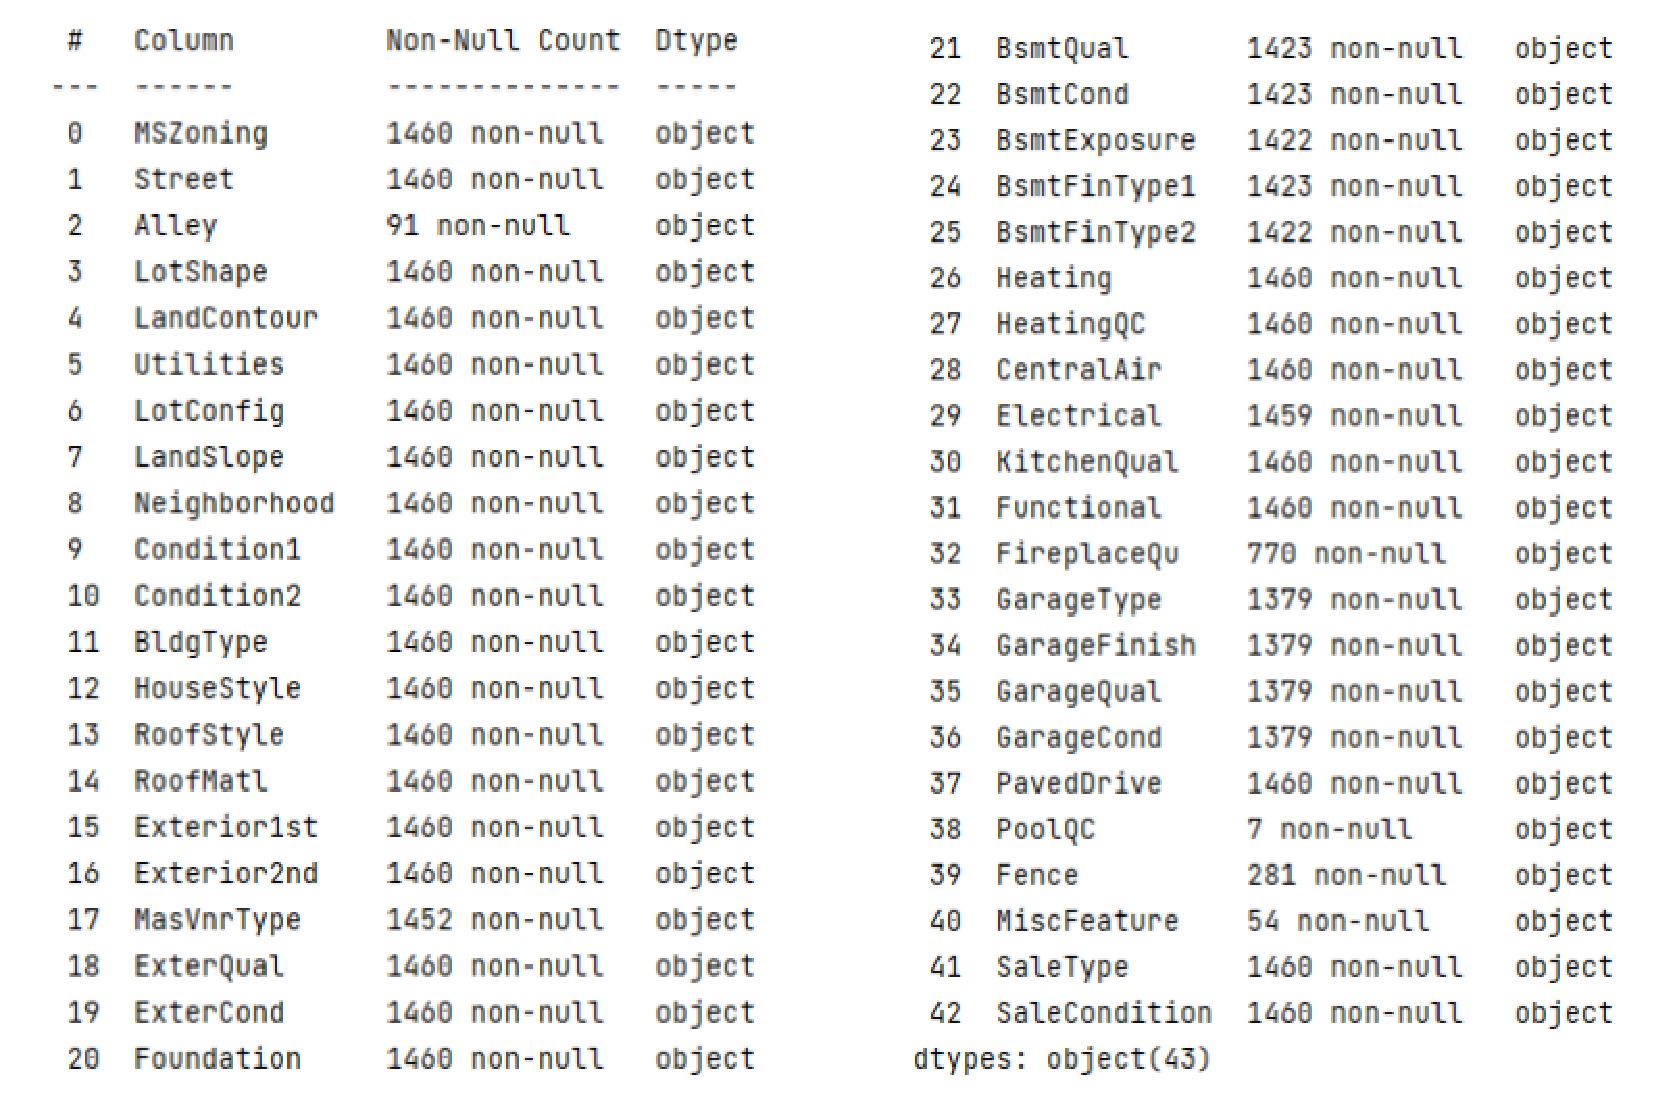
\includegraphics[width=0.65\textwidth]{../Data/Fig1}
		\caption{the variables of type 'object'}\label{object}
	\end{figure}
	The characteristics of variables of type object are represented by string,such as:
	\begin{figure}[H]
		\centering
		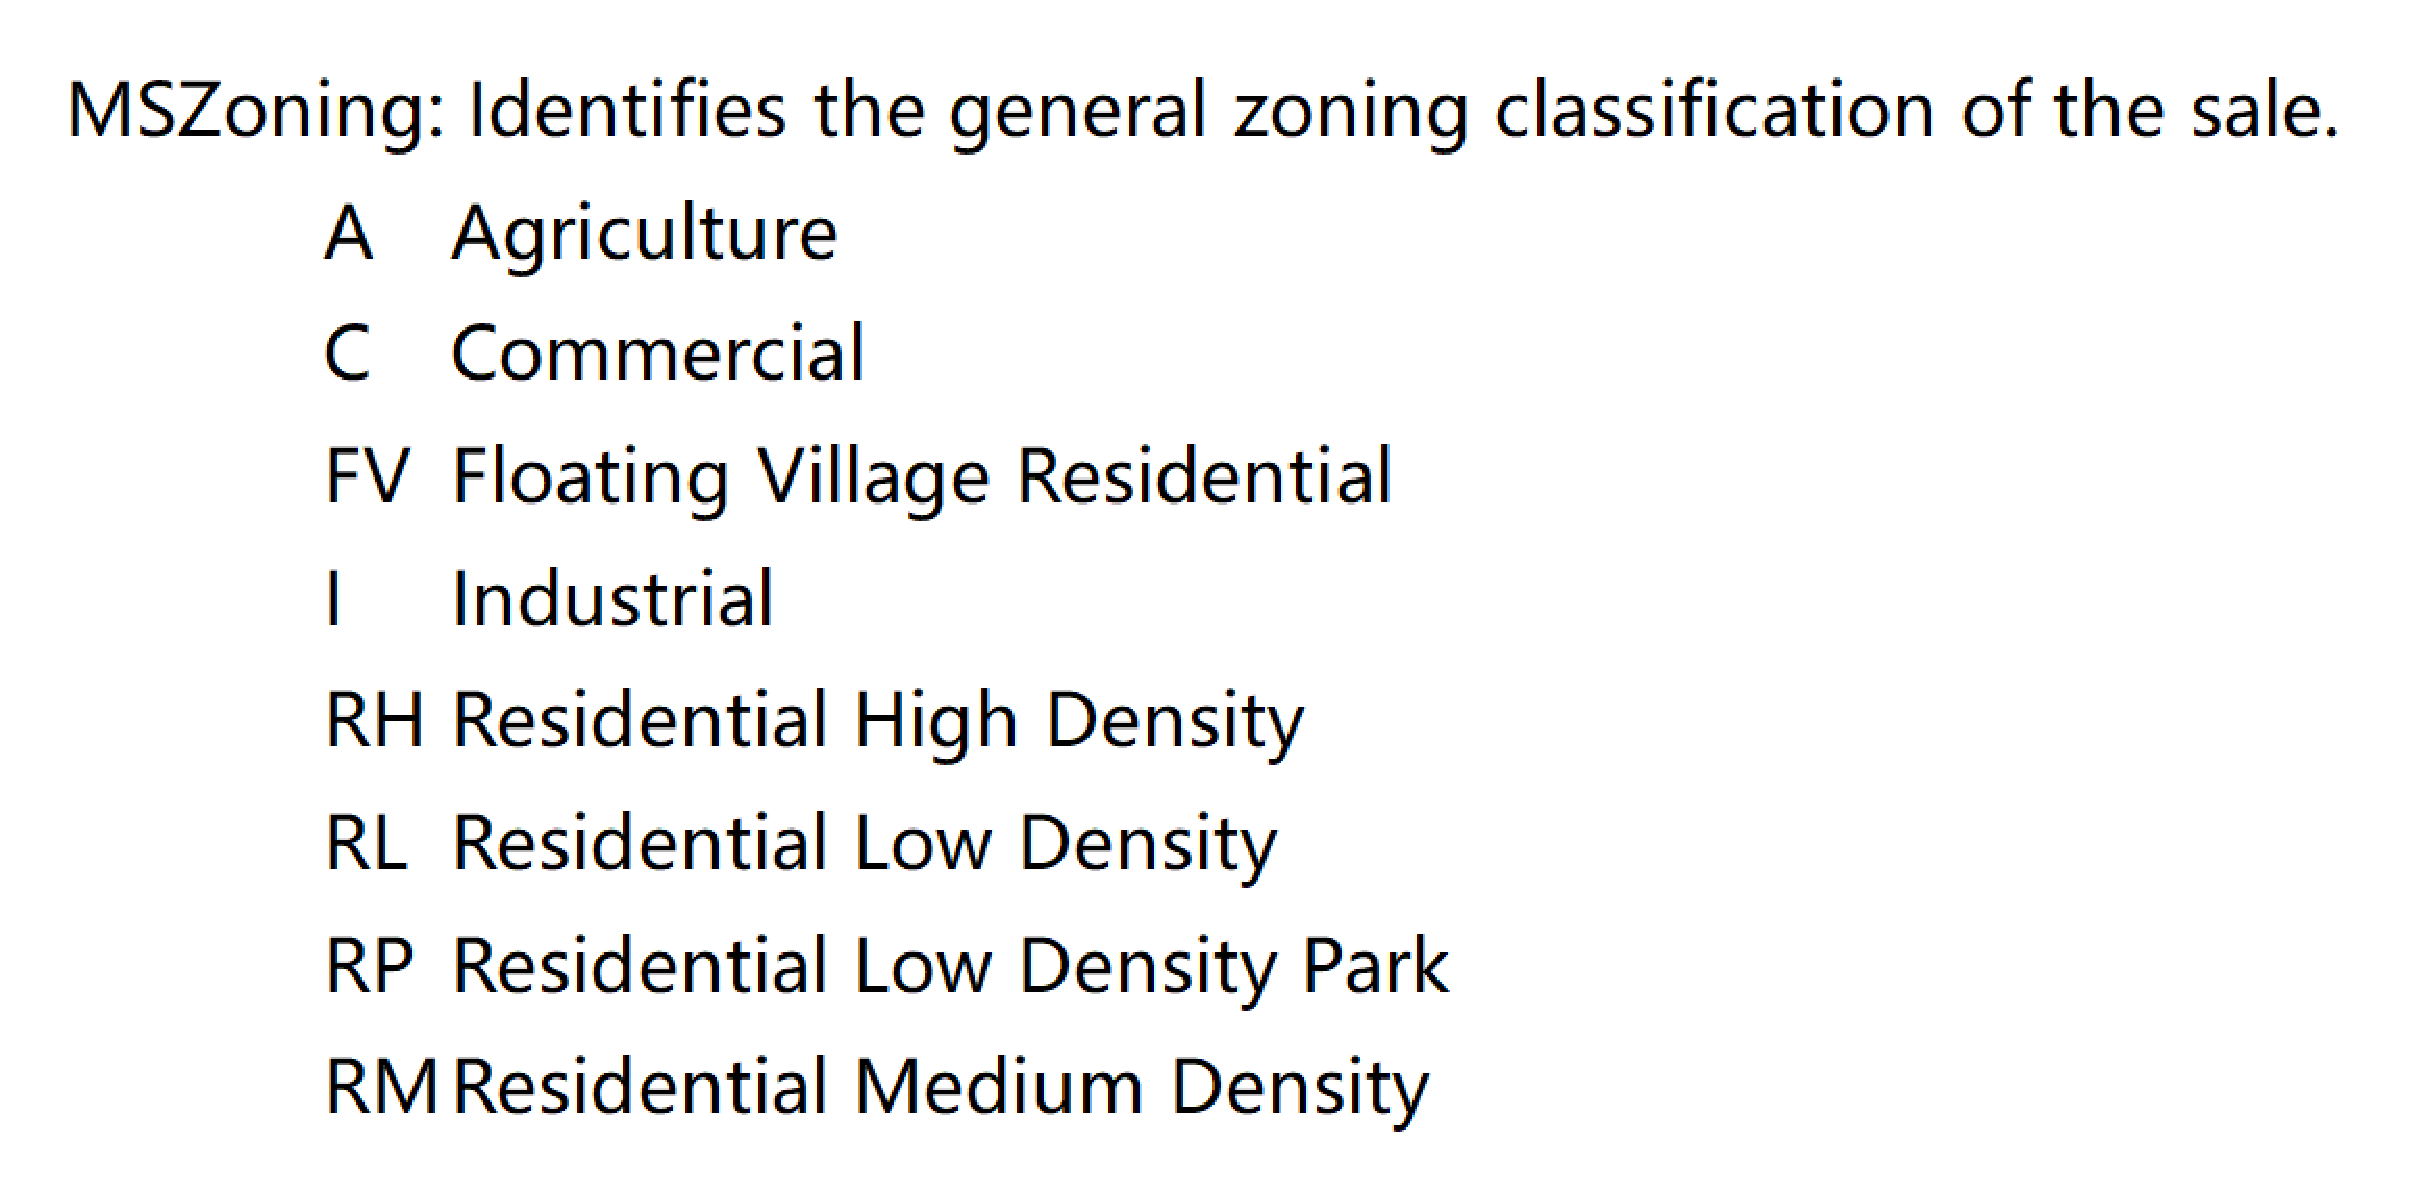
\includegraphics[width=0.6\textwidth]{../Data/Fig2}
		\caption{an example to show the characteristics of type object}\label{object}
	\end{figure}
	The numeric variables are as follows:
	\begin{figure}[H]
		\centering
		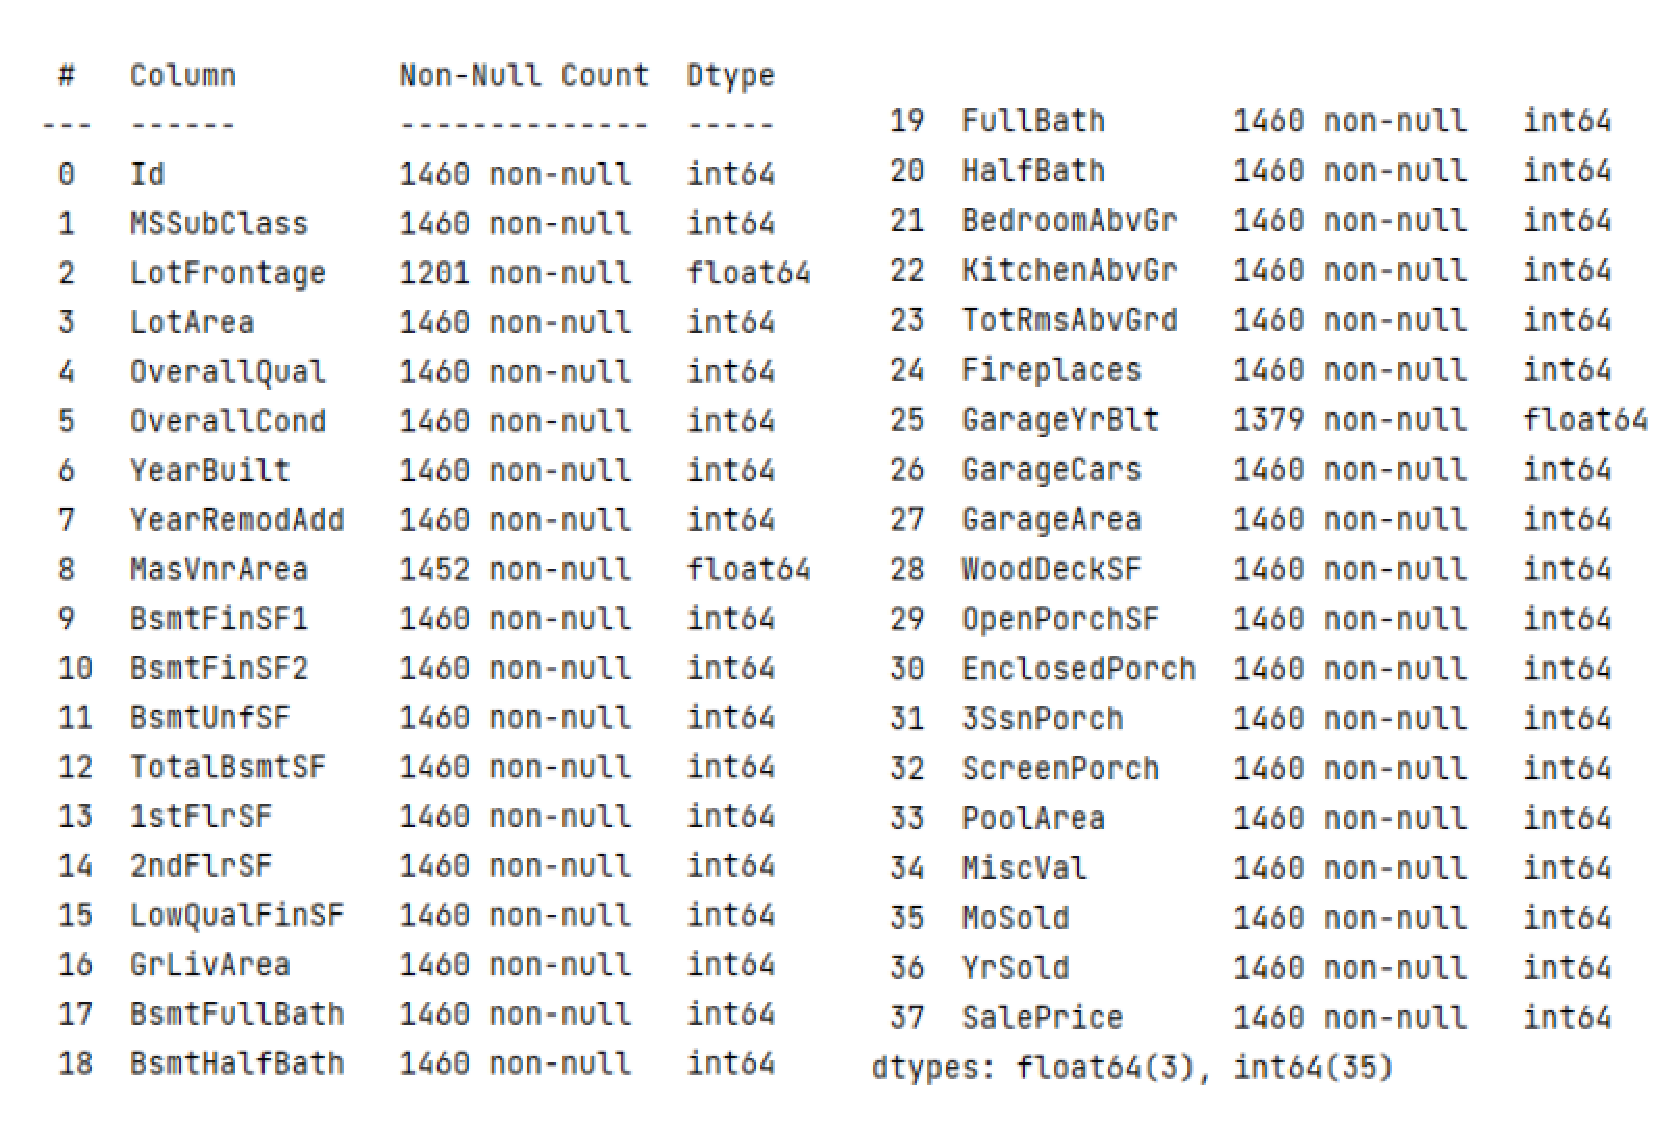
\includegraphics[width=0.65\textwidth]{../Data/Fig3}
		\caption{the variables of type number}\label{object}
	\end{figure}
	\section{Data pre-processing}\label{sec-intro}
	Both the training set data and the test set data have data loss, so we need to perform data cleaning before training. 
	First we count the missing data in the training and test sets, and the  statistics are as follows:
	\begin{itemize}
	\item Number of missing data in the training set:
	\begin{figure}[H]
		\centering
		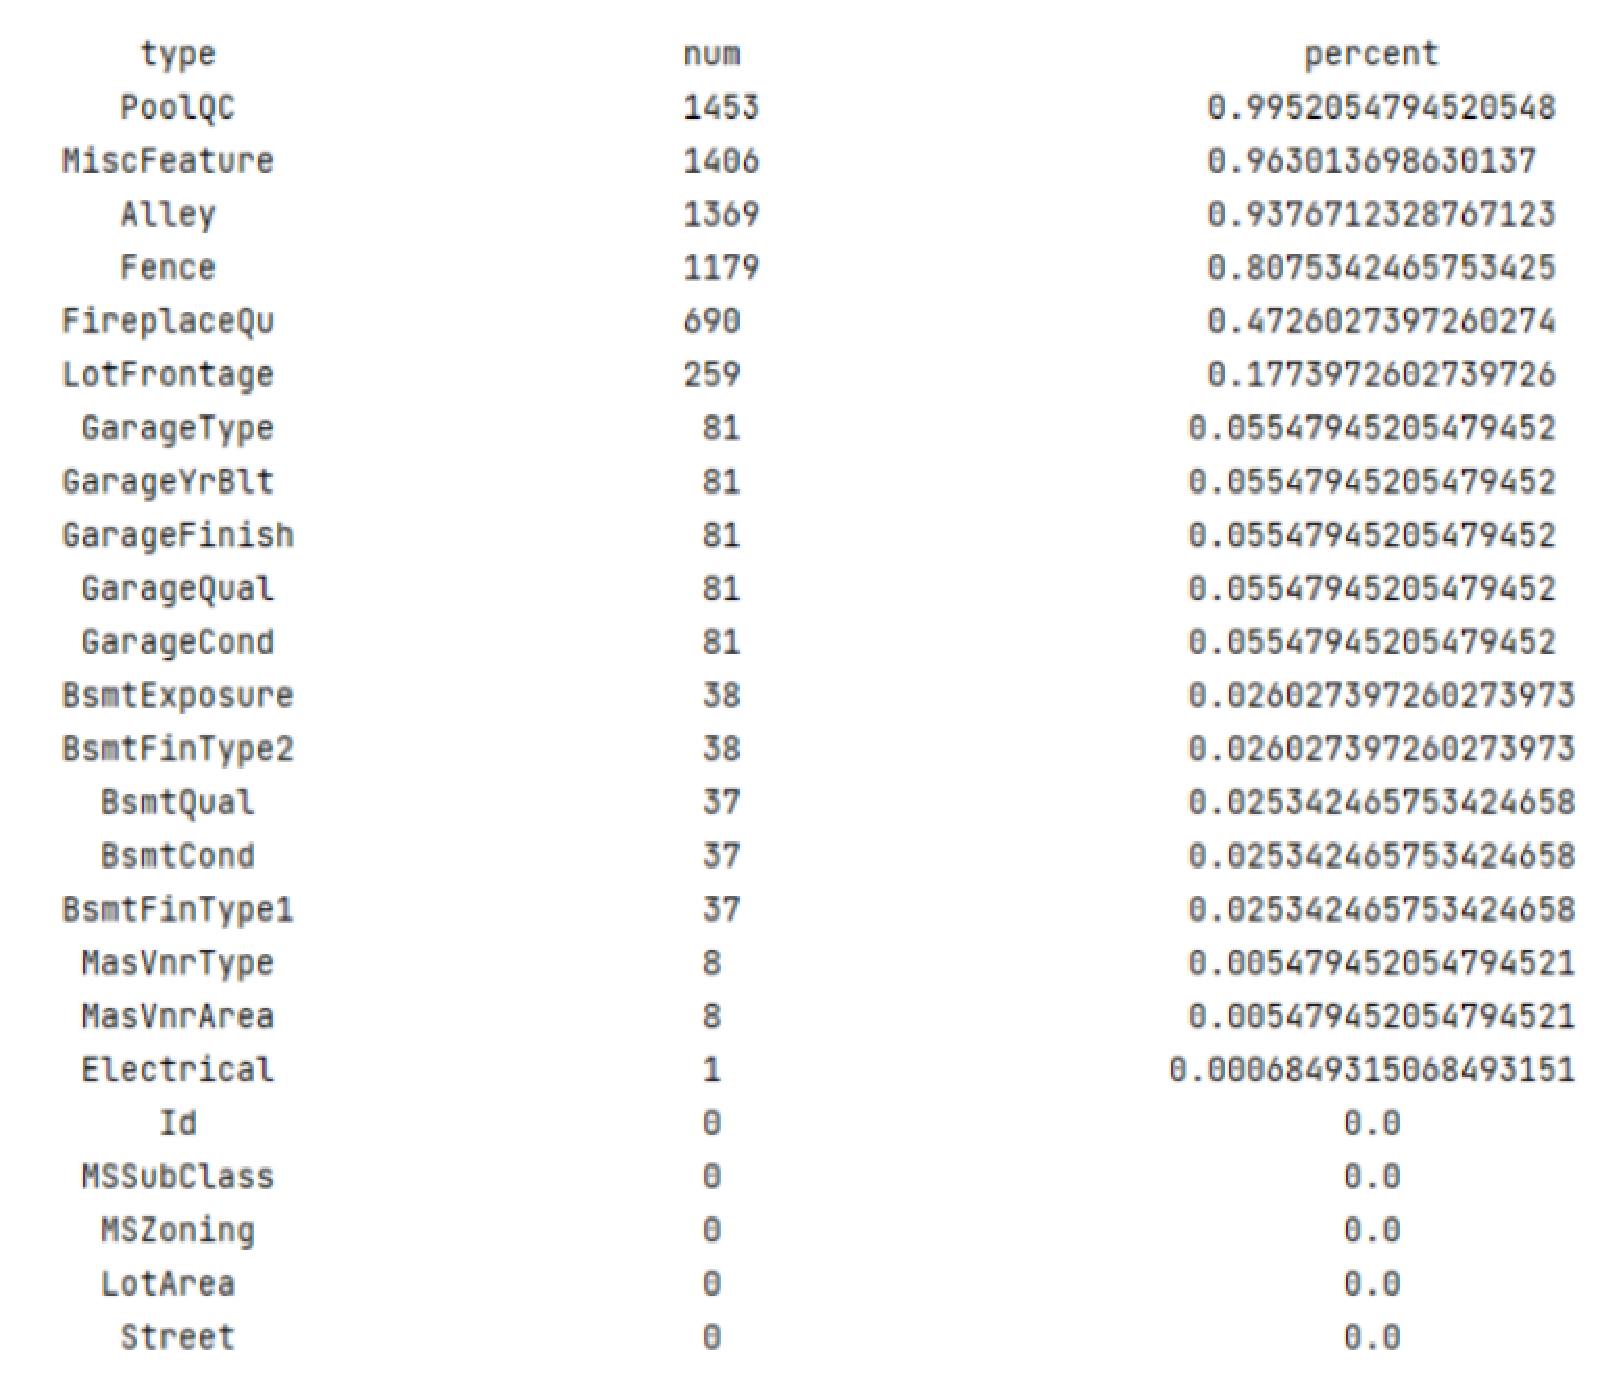
\includegraphics[width=0.55\textwidth]{../Data/Fig4}
		\caption{Number of missing data of training set}\label{object}
	\end{figure}
	\item Number of missing data in the test set:
	\begin{figure}[H]
		\centering
		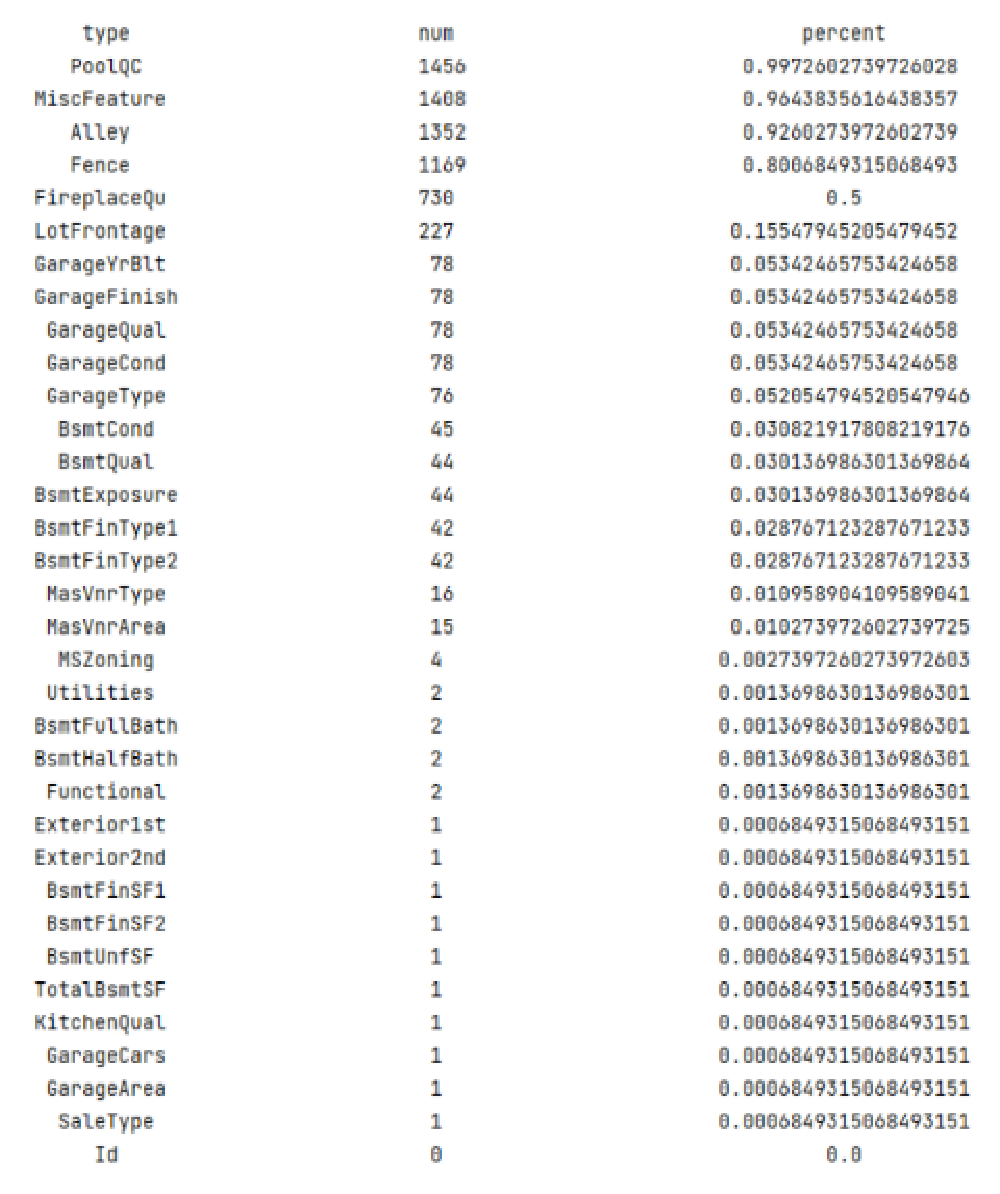
\includegraphics[width=0.55\textwidth]{../Data/Fig5}
		\caption{Number of missing data of test set}\label{object}
	\end{figure}
	\item Data cleaning of training set:\par
	Step2:	Since the properties of numeric types are conveniently complemented by medians or averages, etc., we first examine the properties of numeric types.\par
	\begin{figure}[H]
		\centering
		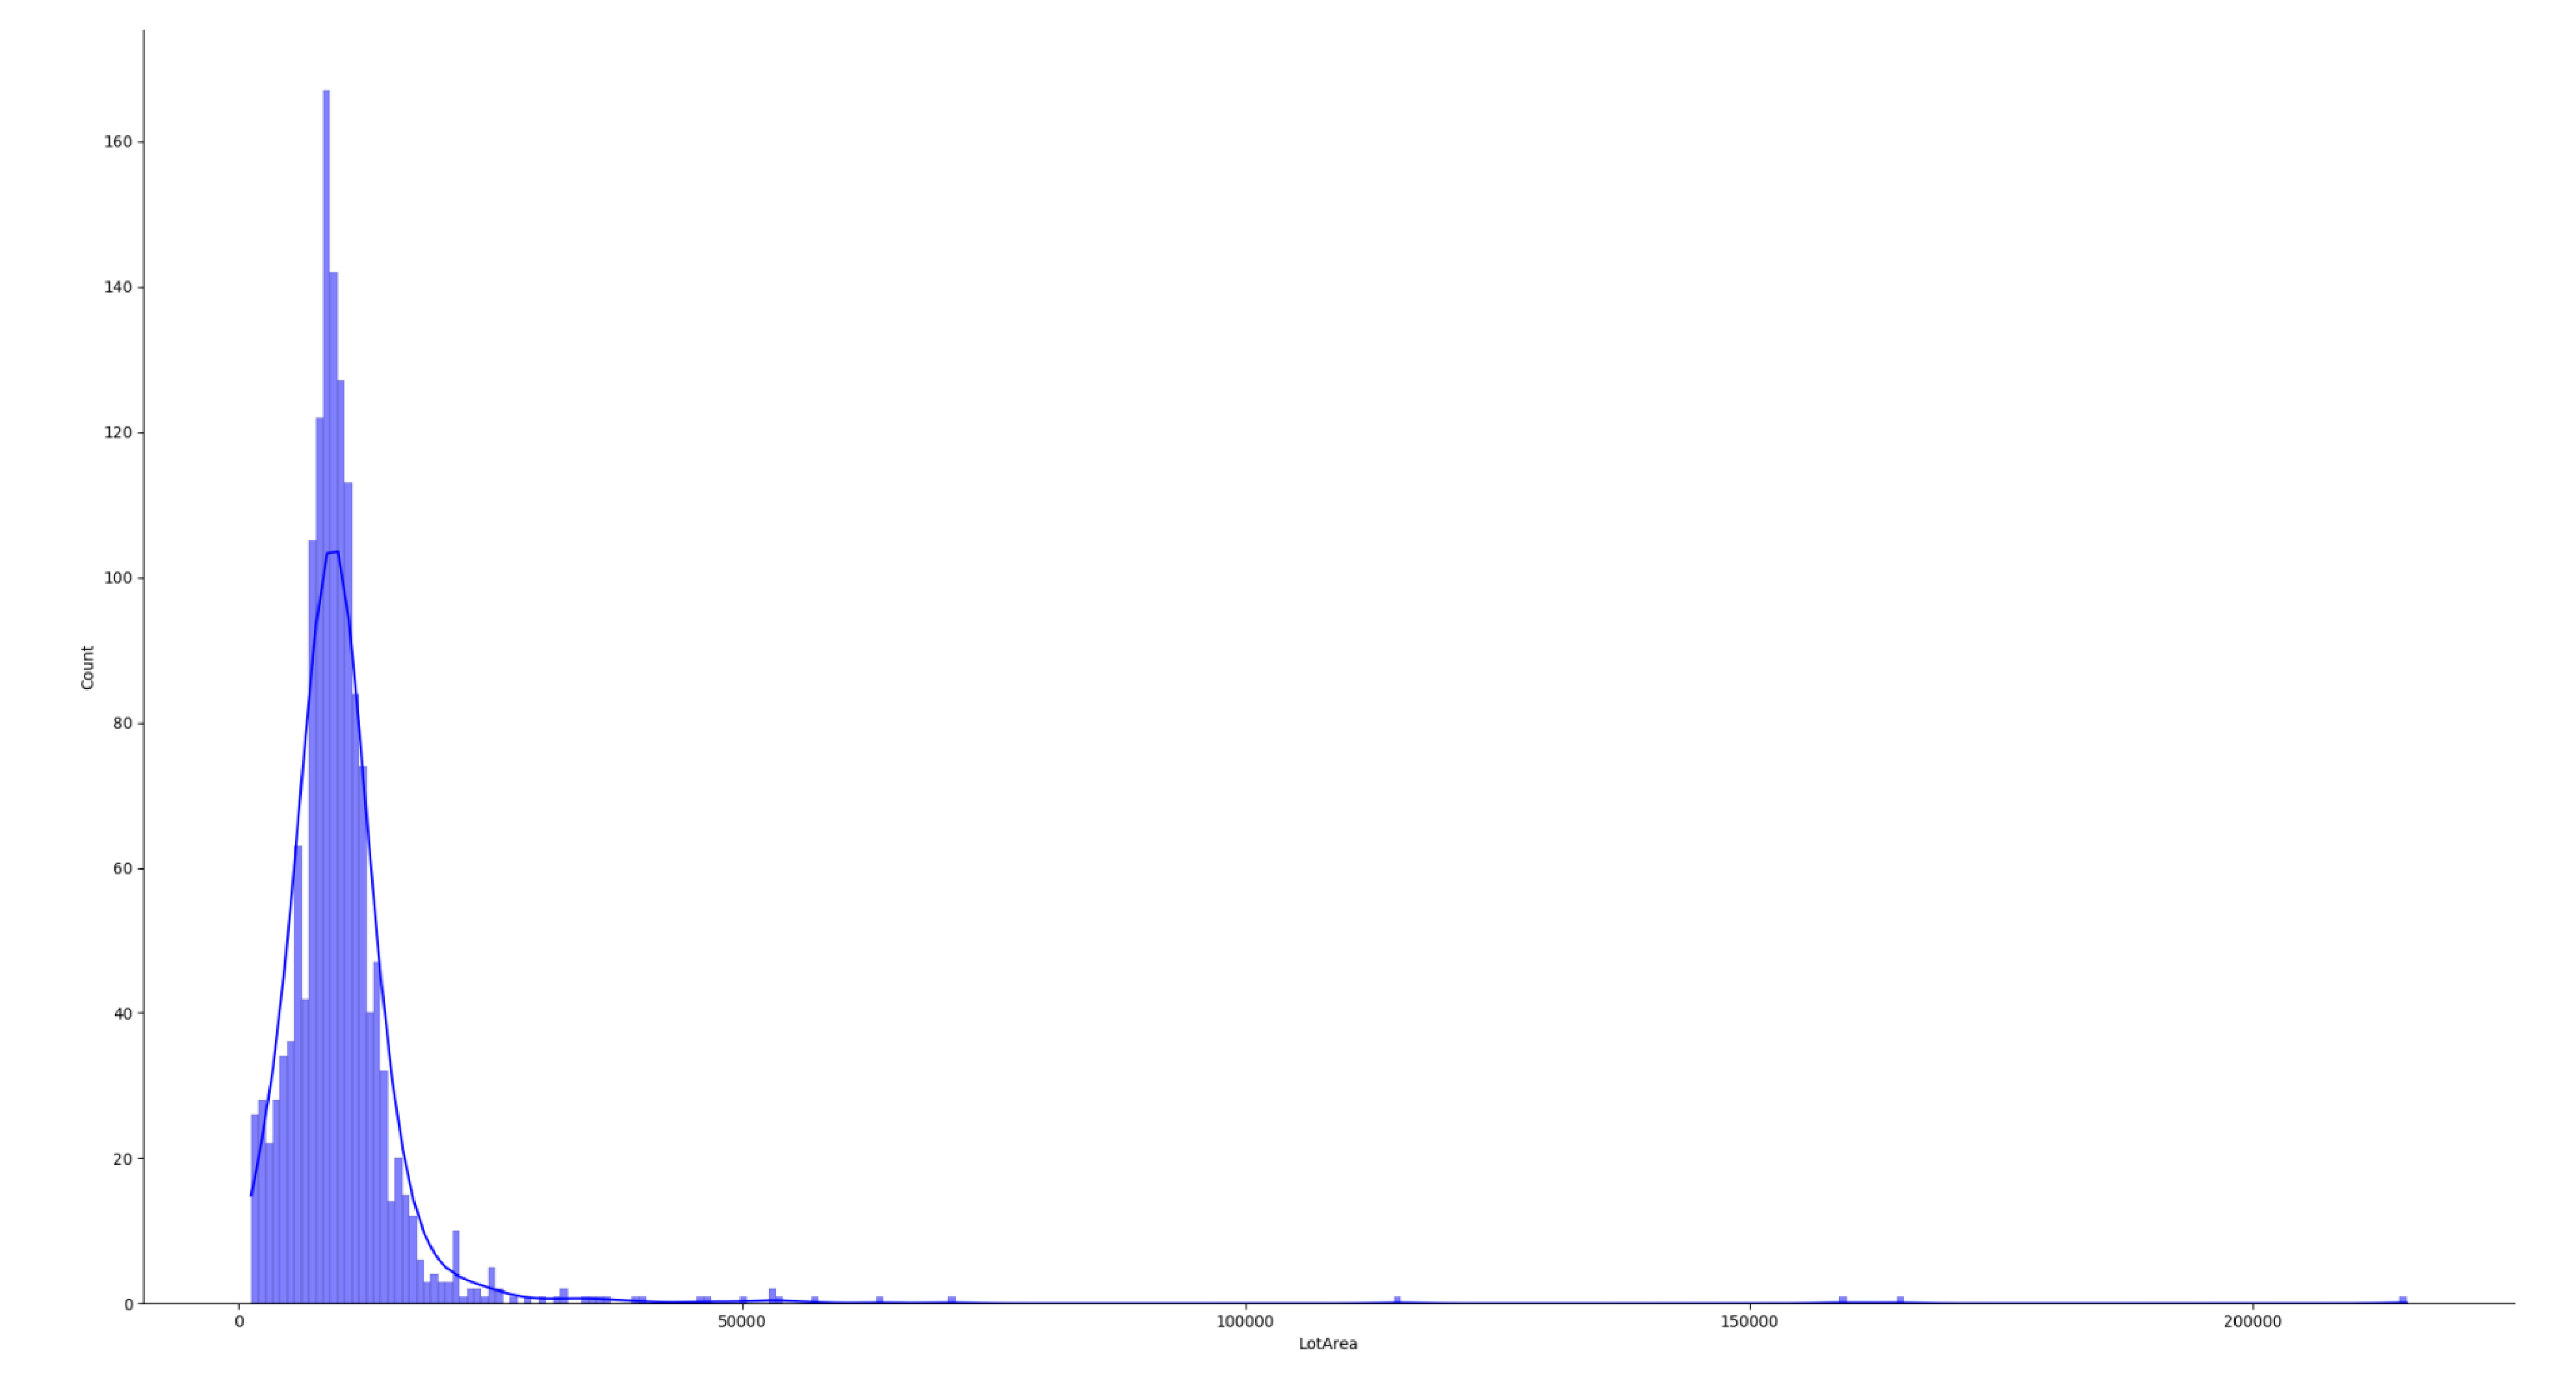
\includegraphics[width=0.85\textwidth]{../Data/Fig6}
		\caption{Positive skew of the feature LotArea}\label{object}
	\end{figure}
	\begin{figure}[H]
		\centering
		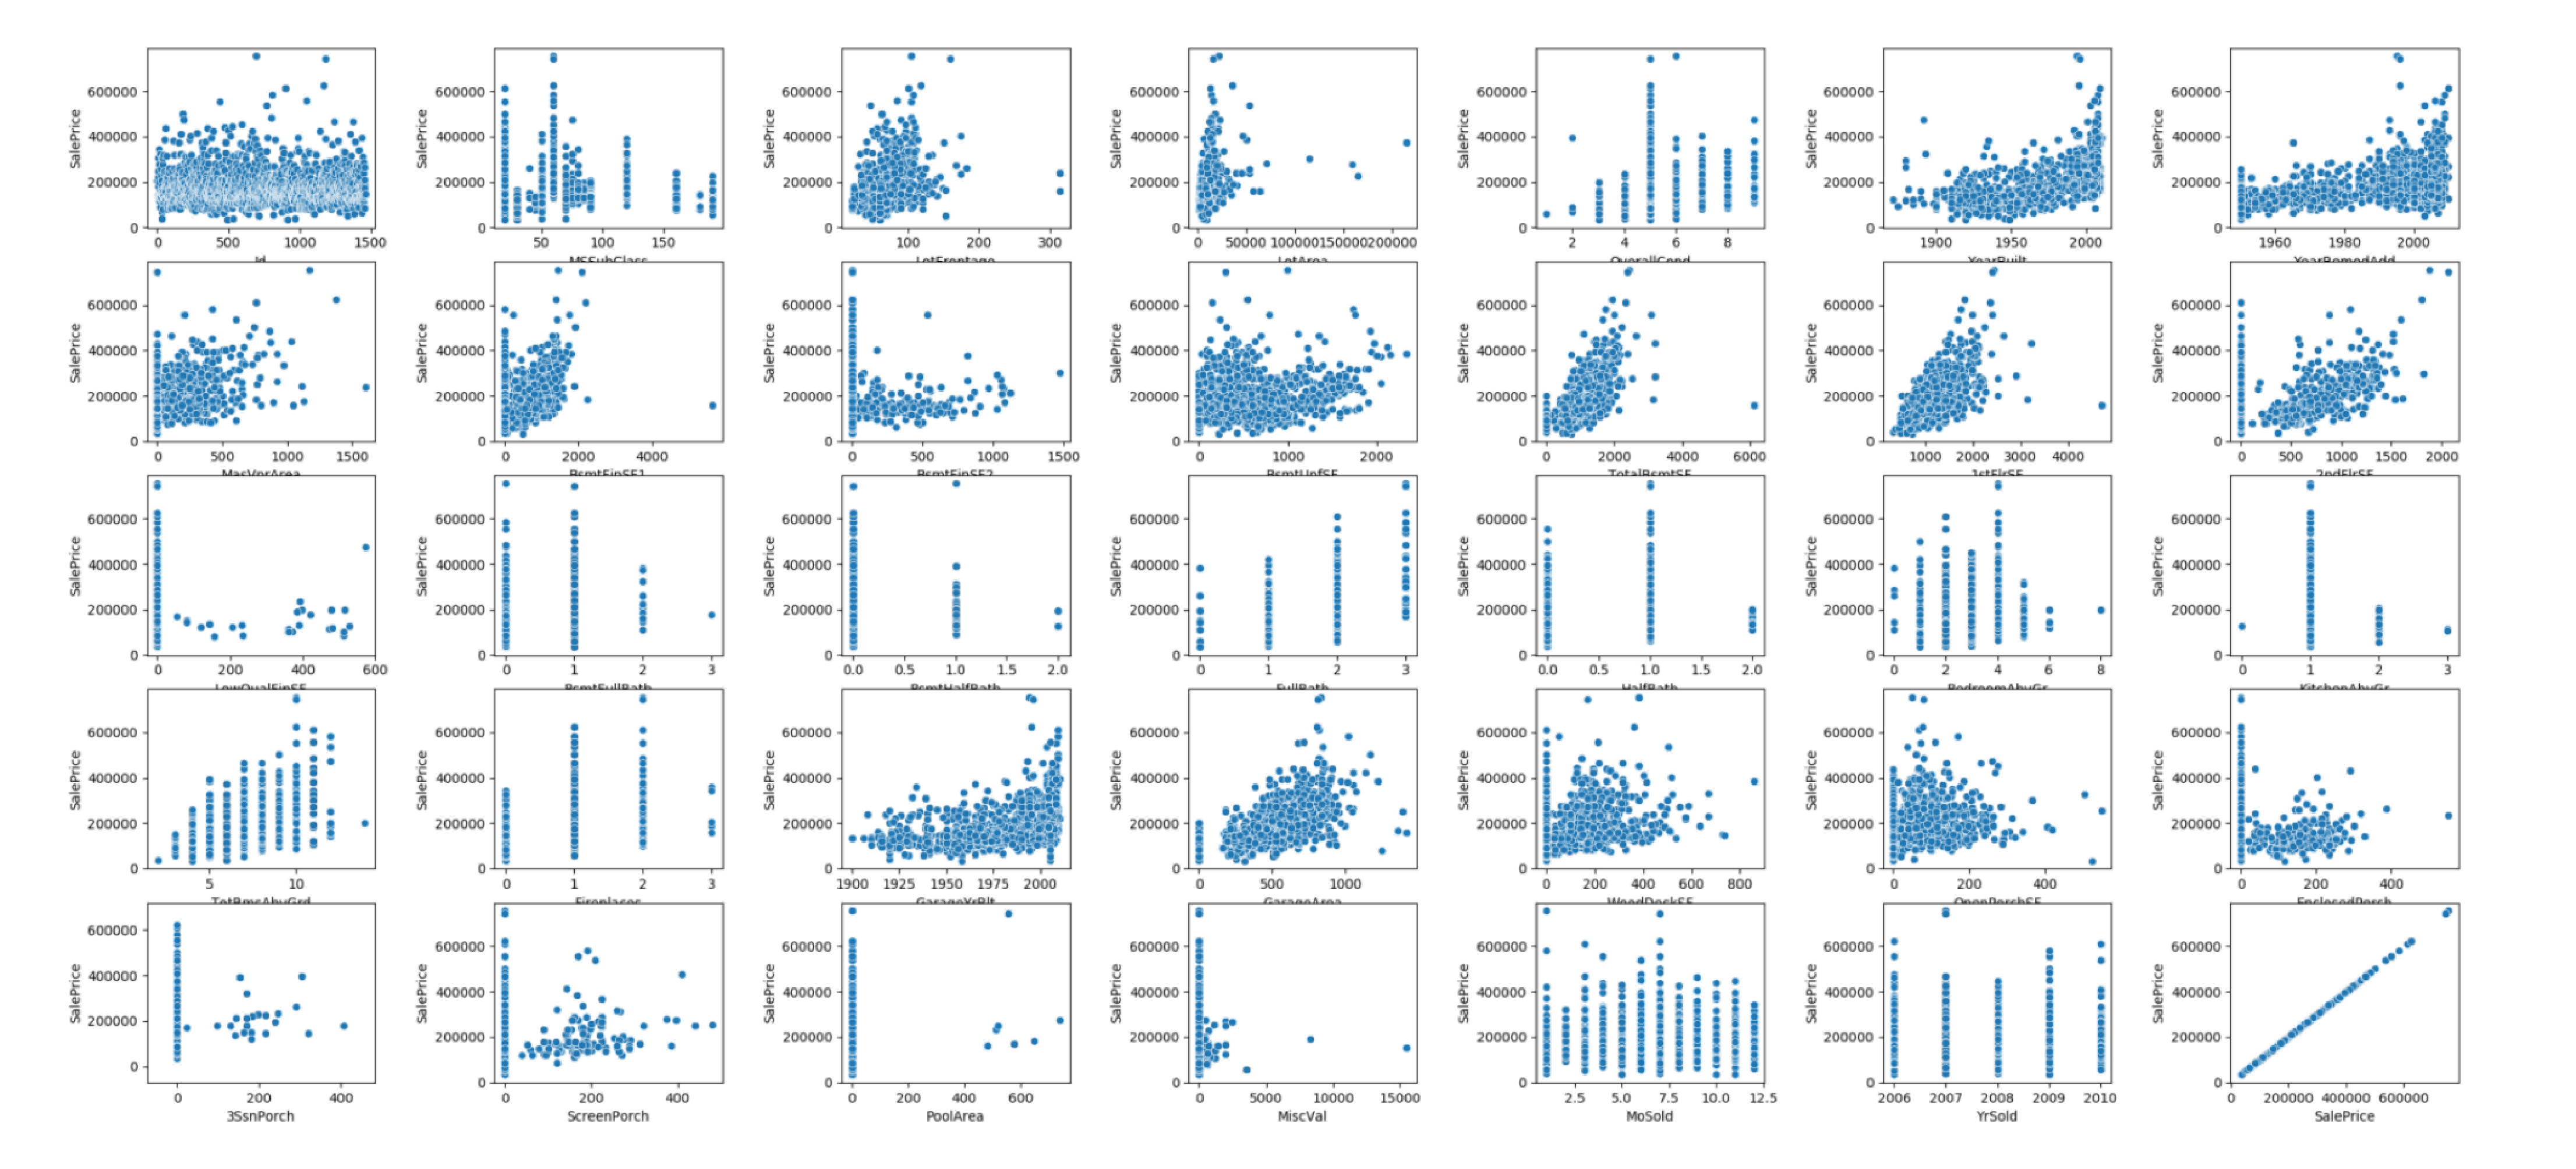
\includegraphics[width=0.9\textwidth]{../Data/Fig7}
		\caption{Data visuallizaion of training data}\label{object}
	\end{figure}
	Step4:Some of the data will be unreasonable, may be too large or too small. We need to remove this data before we put it into the training model. We first use the data visualization to look at it and decide on the removal method in figure7.\par
	From scatter plot we see some columns have outliered data, so drop those rows.\par
	Step5:Now, we analyze the categorical data. For this string type of data, we choose to use the plural to fill in the missing data.\par
	\item Data cleaning of testing set
	All the previous steps are the same, but with the previous steps, we can find that the missing data in the test set is not the same as the training set, so we just need to simultaneously use the same analysis idea for these new missing data.\par
	\item Data normalization and removal of weakly correlated data
	After we clean the training and test set data, we need to consider if all the characteristics are related to the sales price. So we calculate the correlation coefficient of each characteristic and the sales price, we consider the correlation coefficient below 0.3 as almost irrelevant and remove these characteristics
	\end{itemize}
	\section{Training process}\label{sec-intro}
	After cleaning the data, I chose to remove the variables with a correlation coefficient of less than 0.3 with the sales price and put the remaining ones into the linear regression model for training. Now that we have finished pre-processing the data, we need to select the right model for training. I have selected a total of six models to submit.
	\begin{itemize}
	\item Linear Regression
	\par Linear regression models use regression analysis to allow price forecasting by generating a function of saleprice versus variables.After putting the data into the training model, the result given is 0.7313. The submitted data is evaluated based on the root mean square error (RMSE) between the logarithm of the predicted value and the logarithm of the observed sales price. Then 0.7313 is actually a relatively large error, indicating that the linear model is not suitable for house price prediction.
	\item Random Forest
	\par Algorithm flow:
	\par (1)	If there are N samples in the over training sample, then the samples obtained from these N samples are put back for sampling N times and the samples are used for tree building
	\par (2)	Let M be the number of features in the input samples, for each node splitting, we first select m (m<<M) features from these M features, and then select the best splitting point for splitting among these m features
	\par (3)	Each tree is grown as much as possible without pruning
	\par The larger the value of m, the higher the correlation in 1 above and the stronger the classification ability in 2, so m is a very important parameter in RF.
	\par I chose to build 20 decision trees and after putting the training data in, the final training result was 0.16099, which is much better compared to the linear regression model.
	\item K-neighbor
	\par The specific method of the K-nearest neighbor model: with the distance and K values defined in advance, for any new sample, it is classified as the one with the most categories among the K samples with the closest distance to that sample.After putting the data into the model, the prediction result is 0.22111. The k-nearest neighbor method is also okay in predicting house prices, but the accuracy is still not quite enough to be accurate to a range.
	\item Adaboost Regressor
	\par Algorithm flow:
	\par (1)	First obtain the first weak classifier by learning from N training samples.
	\par (2)	Form a new training sample of N by taking the misclassified sample together with other new data, and obtain the second weak classifier by learning from this sample.
	\par (3)	The misclassified samples of 1 and 2 together with other new samples to form a new training sample of N. The third weak classifier is obtained by learning from this sample.
	\par (4)	The final boosted strong classifier. That is, the classification of a data into which category is determined by the classifier weights.
	\par I chose to use 50 decision trees as parameters. After putting the data into the model, the prediction result is 0.22124.The implementation of this algorithm requires a large training sample set in order to achieve higher detection accuracy, and during each iteration, a weak classifier is trained for each sample in that sample set, each sample having many features. However, our data itself is not large and many features are removed, so the final result is mediocre.
	\item Xgboost
	\par Similar to the GBDT routine, XGBoost also requires accumulating the scores of multiple trees to obtain the final prediction score (at each iteration, an additional tree is added to the existing tree to fit the residuals between the prediction results of the previous tree and the true value). xgboost is considered to be an easy-to-use and easily scalable algorithm. After I put the training data in, the training result was rather mediocre and not quite what I thought beforehand, the result was surprisingly 0.60098. I removed the previous operation of removing variables with low correlation coefficients, retrained, and added the number of trees to 400, and then the result became 0.17429. So it was found that in random forest related algorithms, perhaps too many variables should not be removed.
	\item Gradient Boosting Regressor
	\par The gradient boosting algorithm, GBDT mentioned above, was the one that gave me the smallest error in the results during these training sessions. Although xgboost is optimized based on the GBDT algorithm, in this experiment, I was able to achieve 0.15922 after putting in the data, and 0.14173 after keeping the variables with low correlation coefficients as well.
	\end{itemize}
	\section{Conclusion}\label{sec-intro}
	The difference between the house price prediction experiment and the usual data classification is that the data classification only needs to give the data a specific prediction result and then analyze the correct rate. This time, however, the house price prediction is to give the prediction result to a more detailed point, and then to analyze the error. I think this kind of prediction is more difficult to go up to a better result, and the number of data sets itself is not large. I think the training effect can be improved by increasing the dataset through data expansion.
	\par In conclusion, I learned a lot about the new training model in this experiment. For the xgboost model, more adjustments are needed to increase the number of parameters and the depth of the tree to prevent underfitting.
\end{document}